% !TeX program = pdflatex
\documentclass[tikz, border=10pt]{standalone}
\usepackage{tikz}

% --- Définition des styles pour réutiliser les éléments ---
\tikzset{
    % Le style pour la "patate" : notre système physique réel
    system/.style={
        fill=gray!30, 
        draw=black, 
        thick,
        opacity=0.8
    },
    % Le style pour les fonctions candidates du catalogue
    catalog_function/.style={
        draw=blue!80, 
        fill=blue!20, 
        circle, 
        opacity=0.6,
        line width=1pt
    }
}

\begin{document}
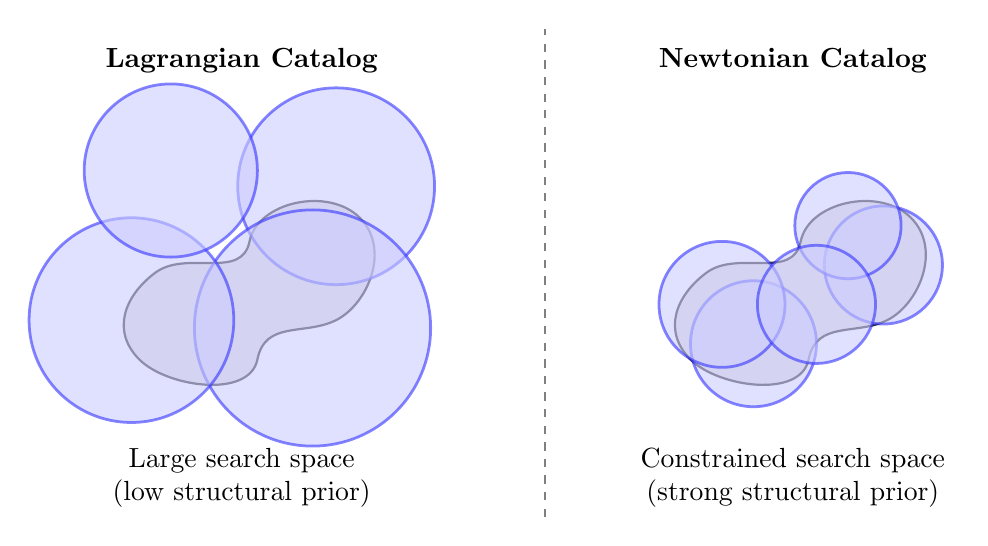
\begin{tikzpicture}

    % --- 1. Dessin du système physique (la patate) ---
    % On le dessine une fois à gauche, et on le réutilise à droite en le décalant
    % Les coordonnées sont choisies pour créer une forme organique et fermée.
    \def\systemshape{
        (0,0) ..controls ++(-45:0.5) and ++(-101.3:0.51) ..  (1.5, 0)
              ..controls ++(78.7:0.51) and ++(-153.4:0.447) .. (2.5, 0.5)
              ..controls ++(26.6:0.447) and ++(-45:0.566) ..  (2.8, 1.8)
              ..controls ++(135:0.566) and ++(78.7:0.51) .. (1.4, 1.5)
              ..controls ++(-101.3:0.51) and ++(36.9:0.5) .. (0.2, 1.1) ..controls ++(-143.1:0.5) and ++(135:0.5) .. (0,0)
    }

    % Système à gauche (Newton)
    \draw[system,xshift=-1cm] \systemshape;

    % Système à droite (Lagrange) - exactement le même, mais décalé de 7 unités
    \begin{scope}[xshift=6cm]
        \draw[system] \systemshape;
    \end{scope}

    % --- 2. Dessin des catalogues de fonctions ---

    % Catalogue Newtonien (Gauche) : large, peu d'information a priori
    % Les cercles sont grands et couvrent une large zone inutile.
    % \node[catalog_function, minimum size=2.8cm] at (0.2, 1.5) {};
    \node[catalog_function, minimum size=2.5cm] at (1.5, 2.2) {};
    \node[catalog_function, minimum size=3cm]   at (1.2, 0.4) {};
    \node[catalog_function, minimum size=2.6cm] at (-1.1, 0.5) {};
    \node[catalog_function, minimum size=2.2cm] at (-0.6, 2.4) {};

    % Catalogue Lagrangien (Droite) : contraint, beaucoup d'information a priori
    % Les cercles sont petits et ciblent parfaitement la forme du système.
    \begin{scope}[xshift=7cm]
        \node[catalog_function, minimum size=1.6cm] at (-0.2, 0.2) {};
        \node[catalog_function, minimum size=1.5cm] at (1.45, 1.2) {};
        \node[catalog_function, minimum size=1.35cm]   at (1, 1.7) {};
        \node[catalog_function, minimum size=1.6cm] at (-0.6, 0.7) {};
        \node[catalog_function, minimum size=1.5cm] at (0.6, 0.7) {};
    \end{scope}

    % --- 3. Ajout des titres et de la séparation ---

    % Titres
    \node[font=\bfseries] at (0.3, 3.8) {Lagrangian Catalog};
    \node[font=\bfseries] at (7.3, 3.8) {Newtonian Catalog};
    \node[below, text width=4cm, align=center] at (0.3, -1) 
        {Large search space \\ (low structural prior)};
    \node[below, text width=4cm, align=center] at (7.3, -1) 
        {Constrained search space \\ (strong structural prior)};

    % Ligne de séparation
    \draw[dashed, thick, gray,xshift=0.65cm] (3.5, -2) -- (3.5, 4.2);

\end{tikzpicture}
\end{document}